\documentclass[10pt]{article}\usepackage[margin=.55in]{geometry}\usepackage[T1]{fontenc}\usepackage{graphicx}\setlength{\parindent}{0pt}\setlength{\parskip}{5pt}\sloppy\begin{document}{\large Retained-session exporter: twelve controls passed}\par Task T-1499. 3 November 2026.\par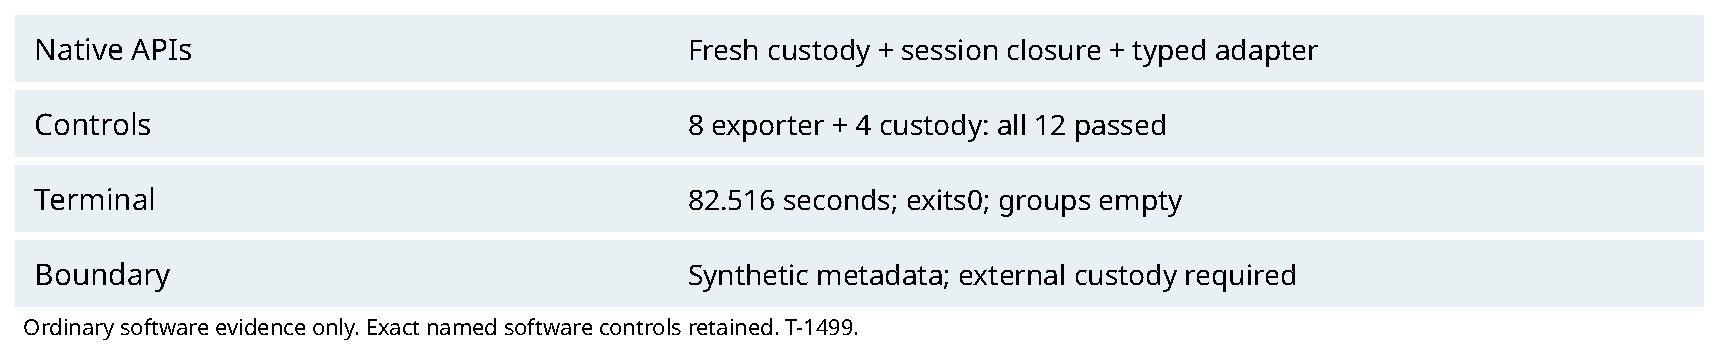
\includegraphics[width=\linewidth]{diagram.pdf}\par The postrun exporter compiled against the coherent native library and passed all twelve named software controls. Eight exporter controls exercise structural acceptance, independent expected pins, native-file mutation rejection, observer semantics, start-time binding, self-asserted controller rejection, prelaunch rejection and symlink rejection. Four inherited custody controls exercise exact external owner, run, configuration, Pod and Job joins.

The exporter calls the actual FreshOwnerPins custody helper, SessionResourceJournal::close\_fresh\_enclosing\_evidence and diagnostic\_file\_adapter::check\_file. Fixtures are synthetic metadata; real controller and worker custody must be supplied independently. The software result establishes these tested acceptance and rejection paths, not authentication of a live controller or admission of a candidate runtime image. Observer worker metrics remain null.

One separately released sequence took 82.515939 seconds within a 120-second ceiling and hard 8 GiB address-space bound. Compiler, test process and outer wrapper exited zero. Both children were reaped with empty process groups; jobserver descriptors closed, no signal or uncertain launch remained. Five source and 888 external inputs matched before and after. The exact twelve unique pass records and zero-failure summary were required, not process exit alone.

The earlier exporter2 compilation failure is preserved separately. This successor changes only fixture construction of the spec identity: the exact four-field canonical object replaces the private identity\_view call. All twelve assertions and actual validators remain unchanged. The native library build is independently preserved in coherent-library-build.

The test binary SHA256 is e75a4db55fd99ed4ba29f65bcb1e6848e8f30ff59ae31e82fd9e738bdd9f0e9f. Receipt SHA256 is 3220d130f8cf72872a1e7dddcf7784bd9514cb70161c1d6051768bd6aca30e3b. Exact source, commands, named outcomes and warnings are retained in the evidence archive.
\end{document}